\section{Itération 1: ( 2/22/2017 - 3/5/2017 )}

\subsection{Objectif de l'itération}
L'objectif de cette itération est d'étudier notre Serveur ,de générer notre modèle,de réaliser
la page Web (dashboard) et développer les vues nécessaires pour permettre à l'utilisateur
de consulter la dernière position du véhicule selon les spécifications du Backlog.\\
Une fois la première ébauche du Backlog est réalisée, le product owner peut découper
les spécifications de haut niveau vers des spécifications plus raffinées. Dès lors nous
passons à la planification d’une itération. Il est important de rappeler que les premières
spécifications du Backlog doivent être:
\begin{itemize}
 \item assez précise pour être estimée par l’équipe
 \item assez petite pour être développée et testée durant une itération
\end{itemize}
Ayant une bonne idée sur le produit ainsi que l’objectif à atteindre, l’équipe et le
product-owner peuvent passer à l’élaboration des itérations.
Dans notre projet ``Plateforme CityWatch'' la durée d’une Itération est fixée à trois
semaines (170h par itération). Dans ce chapitre nous décrivons le déroulement des deux
premières itérations. Une itération commence par sa planification et finit par être revue
avec ”Product-Owner”.

\subsection{Planification de l'itération}

Dans le but de définir le périmètre fonctionnel de l'itération 1 et faire
sa planification, tous les membres de l'équipe ont participé à un réunion
avec le Scrum Master et le Product Owner pour définir le backlog du sprint.\\

La planification de l'itération représente une étape importante dans la vie de
l'itération parce que au cours du planification, on divise l'itération a plusieurs étapes
pour mieux atteindre le résultats attendu à la fin de l'itération.
Dans cette première itération on a décidé de diviser cette dernière en trois grandes
parties une partie consacrée pour la création de la base de donnée et la génération du
modèle, la deuxième partie est consacré pour la réalisation de la page d’accueil, et une
troisième partie qui répond aux besoins des autres tâches de cette itérations.

\subsubsection{Préparation de la liste des tâches }
Les tâches à réaliser peuvent être soient des tâches de recherche, de documentation, de
conception, de développement ou bien d’installation, de tests, d’intégration...etc.
Il est recommandé lors de la planification de la liste des tâches de bien les détailler. Une tâche
ne doit pas inclure d’autres tâches. Ceci permet de bien cerner le travail demandé.
\begin{center}
    \footnotesize
    \begin{longtable}{| p{1cm} | p{5cm} | p{7cm} | p{1cm} |}
        \caption{Taches à faire de la première itération}
        \label{tab:sprint1-backlog} \\

 \hline
 \textbf{Réf} & \textbf{Spécification} & \textbf{Description} & \textbf{Priorité} \\ \hline
 \endhead

 \hline \multicolumn{4}{|r|}{{Continué en page suivante$\dotsc$}} \\ \hline
 \endfoot

 \hline \hline
 \endlastfoot

\hline
1 & Présentation et Configuration SVN & Présenter SVN, installer le serveur SVN et créer les répertoires  & 1 \\ \hline
2 & Recherche sur les Services Web & Présenter les différentes Solutions des services web et choisir la meilleur solution & 1 \\ \hline
3 & Implémenter service Save Position & Enregistrement les coordonnées requis dans la base de données & 2 \\ \hline
4 & Implémenter la consommation du service Save Position & Coordonnées enregistrés instantané et continuellement dans la BD & 1 \\ \hline
5 & Recherche sur les spécifications de la plateforme Android & Présenter le modèle de développement Android et choisir le SDK optimale & 1 \\ \hline
6 & Création Application Template minimal & Application fonctionnel et intégration au SVN & 1 \\ \hline
7 & Implémenter service Get Last Position & Le serveur retourne les dernières coordonnées requis & 1 \\ \hline
8 & Rectification service Save Positon & Support multiple périphériques et enregistrer la date d'envoyé & 2 \\ \hline
9 & Rectification service Get Last Position & Retourné la position du périphérique et la date du dernier modification & 2 \\ \hline
10 & Affiche Multiple marqueurs & Afficher dernière position de chaque périphérique dans la carte & 2 \\ \hline
11 & Affiche état du périphérique & Afficher si le périphérique est en ligne ou hors ligne & 3 \\ \hline
\end{longtable}
\end{center}

\subsubsection{Estimation de la première itération}

Nous avons fixé la période d’une itération à 3 semaine. Dans
cette section, nous présentons une estimation du nombre d’heures pendant lesquelles
nous nous engageons à travailler.

\begin{table}[htbp]
    \centering
    \begin{tabular}{| c | c | c | c |}
\hline
\textbf{Membre} & \textbf{Nombre d'heures par jour} & \textbf{Nombre de jours présent} & \textbf{Total en heures} \\ \hline
\hline

Moez & 6 & 10 & 60\\ \hline
Rihab & 6 & 10 & 60 \\ \hline
\multicolumn{2}{c|}{} & \textbf{Total} & 120 \\ \cline{3-4}
    \end{tabular}
    \caption{Nombre d'heures de travail estimé de l'itération 1}
    \label{tab:sprint1-capacity}
\end{table}

\begin{center}
    \begin{longtable}{| l | l | l |}
        \caption{Nombre d'heures estimé pour la réalisation des taches}
        \label{tab:sprint1-estimation} \\

 \hline
 \textbf{Spécification} & \textbf{Membre} & \textbf{Heures} \\ \hline
 \endhead

 \hline \multicolumn{3}{|r|}{{Continué en page suivante$\dotsc$}} \\ \hline
 \endfoot

 \hline \hline
 \endlastfoot

\hline
Présentation et Configuration SVN & Rihab & 5 x 2 \\ \hline
Recherche sur les Services Web & Moez & 13 x 2 \\ \hline
Implémenter service Save Position & Moez & 5 \\ \hline
Implémenter la consommation du service Save Position & Rihab & 5 x 2 \\ \hline
Recherche sur les spécifications de la plateforme Android & Rihab & 13 x 2 \\ \hline
Création Application Template minimal & Rihab & 13 \\ \hline
Implémenter service Get Last Position & Moez & 5 \\ \hline
Rectification service Save Positon & Moez & 5 \\ \hline
Rectification service Get Last Position & Moez & 5 \\ \hline
Affiche Multiple marqueurs & Moez & 5 \\ \hline
Affiche état du périphérique & Rihab & 5 \\ \hline
\end{longtable}
\end{center}	

\subsection{Présentation des outils utilisés}

Le stage chez Djagora Academy nous a permis d'acquérir de nouvelles
compétences tant au nivrau relationnel que technique.Pour bien entamer la réalisation
de la plateforme 
``City Watch''nous avons suivi différentes
formations sur les outils et les technologies que nous venons de citer. 

\subsubsection{Apache Subversion}

Un logiciel de gestion de versions est un logiciel de gestion de configuration
permettant de stocker des informations pour une ou plusieurs ressources
informatiques permettant de récupérer toutes les versions intermédiaires des
ressources,vainsi que les différences entre les versions.

Apache Subversion (en abrégé SVN) est un logiciel de gestion de versions,
distribué sous licence Apache et BSD.
VisualSVN est un plug-in d’intégration de Subversion de qualité professionnelle.
Les principaux avantages de VisualSVN sont les suivants:

\begin{itemize}
    \item Fiabilité imbattable : Visual Studio ne s’arrêtera jamais ni ne
        s’arrêtera à cause de VisualSVN.
    \item Intégration transparente : VisualSVN gère automatiquement les fichiers
        ajoutés ou renommés et reflète ces opérations sur Subversion.
    \item Statut en temps réel : VisualSVN suit attentivement et affiche toutes
        les modifications apportées à votre copie de travail.
    \item Courbe d’apprentissage courte : VisualSVN utilise les boîtes de
        dialogue TortoiseSVN et fournit un assistant intelligent pour mettre
        vos sources sous Subversion.
\end{itemize}
VisualSVN Server vous permet d’installer et de gérer facilement un serveur
Subversion entièrement fonctionnel sur la plateforme Windows. Il est utile tant
pour les petites entreprises que pour les entreprises.

\subsubsection{Android}

Android est un système d'exploitation conçu en 2007 par la societé Android,
start-up racheté par Google . Android est Open Source, ca veut dire on peut lire
le code de ce logiciel le modifier et le redistribuer.

Les bases que nous utilisons:

\paragraph{IDE:}

C'est un logiciel dont son objectif est de faciliter le développement. Il est
toujours possible de développer une application sans IDE.
l'IDE est constitué d'outils dont au moins un éditeur de texte.
On utilisera dans notre projet l'IDE Android Studio, l'IDE privilège de Google.
Android Studio comporte l'auto-complétion la génération automatique  du code des
outils de compilation et débogage et plusieurs autres services qui permettent de
développer une application facilement et rapidement.

\paragraph{SDK:}

C’est une abréviation qui peut faire référence a Software Developpement Kit.
Les applications Android sont développés en JAVA. Un appareil Android ne
comprend pas le langage JAVA, il comprend une variante de JAVA adaptée pour lui.
On a recours ici SDK, c'est ensemble des outils permettant de développer dans
une cible particulière. Un SDK Android est alors un ensemble des outils qui
permettent de développer des application pour Android.

\paragraph{Activity:}

Un utilisateur habile d'Android remarque que lors de l'exploitation d'une
application Android qu'il est en train de naviguer entre des fenêtres et
l'application ne afficher qu'une seule fenêtre à la fois ces fenêtre la sont
des activités on peut différencier ces activité a travers leur interface
graphique ceci s'applique sur la plupart des application Android car il y a
des applications qui contiennent pas d'activités. Un première idée qui nous
frappe la tète c'est que une activité est un conteneur d'élément graphique qui
constitue un interface graphique. Alors que ne non une activité n'est pas
seulement une interface graphique mais elle va établir les liens entre
l'interface graphique et la logique programma tique de plus l'activité
contient des informations sur le statut actuel de l'application qui s'appelle le
contexte ce contexte permet de faire la liaison entre le système Android et les
autres activities de l'application.

\subparagraph{États d'activities:}

Le système Android met en place un système priorités entre application
par exemple l'utilisateur est en train de naviguer sur internet et écouter
de la musique il reçois un appel comme l'application qui gère les appel est
une application plus prioritaire elle prend la du navigateur et le lecteur
musique pour que l'utilisateur puisse répondre a son appel. Si une application
consomme trop de ressources et peut bloquer le fonctionnement du système Android,
Android arrêtera cette application. Et aussi comme expliqué précédemment
les activités sont gères a partir d'un système de pile d'activités .
D'où l'apparition de plus d'un état qui sont centré sur l'activité.

On peut différencier ces états par leur visibilité :
\begin{itemize}
 \item État Active
 \item État Paused
 \item État Stopped
\end{itemize}

\subparagraph{Cycle de vie d'une activité :}

Une activité n'a pas de contrôle sur son état.
Son état change suivant un cycle rythmique entre le système Android et les
AUTres application (un système quasi dépendant sur des priorités comme expliqué
précédemment) la figure~\ref{fig:android-activity} explique le cycle de vie
d'une activité. (Les états sont représenter comme des méthodes parce que lors de
la programmation ces états sont interroges par le nom de ces méthodes.\\
la figure~\ref{fig:android-activity} représente le cycle de vie d'une activité.

% Diagram of Android activity life cycle
% Author: Pavel Seda 
% Drawing part, node distance is 1.5 cm and every node
% is prefilled with white background
\begin{figure}[H]
 \centering
 \footnotesize

\begin{tikzpicture}[node distance=1.5cm,
    every node/.style={fill=white, font=\sffamily}, align=center]
  % Specification of nodes (position, etc.)
  \node (start)             [activityStarts]              {L'activité démarre};
  \node (onCreateBlock)     [process, below of=start]          {onCreate()};
  \node (onStartBlock)      [process, below of=onCreateBlock]   {onStart()};
  \node (onResumeBlock)     [process, below of=onStartBlock]   {onResume()};
  \node (activityRuns)      [activityRuns, below of=onResumeBlock]
                                                      {Activity is running};
  \node (onPauseBlock)      [process, below of=activityRuns, yshift=-1cm]
                                                                {onPause()};
  \node (onStopBlock)       [process, below of=onPauseBlock, yshift=-1cm]
                                                                 {onStop()};
  \node (onDestroyBlock)    [process, below of=onStopBlock, yshift=-1cm] 
                                                              {onDestroy()};
  \node (onRestartBlock)    [process, right of=onStartBlock, xshift=4cm]
                                                              {onRestart()};
  \node (ActivityEnds)      [startstop, left of=activityRuns, xshift=-4cm]
                                                        {Le processus est tué};
  \node (ActivityDestroyed) [startstop, below of=onDestroyBlock]
                                                    {l'activité est arrêtée};     
  % Specification of lines between nodes specified above
  % with aditional nodes for description 
  \draw[->]             (start) -- (onCreateBlock);
  \draw[->]     (onCreateBlock) -- (onStartBlock);
  \draw[->]      (onStartBlock) -- (onResumeBlock);
  \draw[->]     (onResumeBlock) -- (activityRuns);
  \draw[->]      (activityRuns) -- node[text width=4cm]
                                   {Une autre activité s'intercole devent notre activité} (onPauseBlock);
  \draw[->]      (onPauseBlock) -- node {Notre activité n'est plus visible}
                                   (onStopBlock);
  \draw[->]       (onStopBlock) -- node {L'activité est arrêtée par le système ou l'utilisateur} (onDestroyBlock);
  \draw[->]    (onRestartBlock) -- (onStartBlock);
  \draw[->]       (onStopBlock) -| node[yshift=1.25cm, text width=3cm]
                                   {L'activité revientsur le devant de la scène}
                                   (onRestartBlock);
  \draw[->]    (onDestroyBlock) -- (ActivityDestroyed);
  \draw[->]      (onPauseBlock) -| node(priorityXMemory)
                                   {Priorité élevée $\rightarrow$ plus mémoire}
                                   (ActivityEnds);
  \draw           (onStopBlock) -| (priorityXMemory);
  \draw[->]     (ActivityEnds)  |- node [yshift=-2cm, text width=3.1cm]
                                    {L'utilisateur retourne vers l'activité}
                                    (onCreateBlock);
  \draw[->] (onPauseBlock.east) -- ++(2.6,0) -- ++(0,2) -- ++(0,2) --
     node[xshift=1.2cm,yshift=-1.5cm, text width=2.5cm]
     {L'activité revient sur le devant de la scéne}(onResumeBlock.east);

  \end{tikzpicture}
  \caption{Diagramme de cycle de vie d'activite Android}
  \captionsource{Pavel Seda, \TeX example.net [Modifié]}{http://www.texample.net/tikz/examples/android/}
  \label{fig:android-activity}
\end{figure}


\subparagraph{Comment choisir le SDK optimale :}

Une SDK permet l'application de marcher sur la version Android visé
et les versions ultérieure il  a noté de prendre en considération le taux des
utilisateurs visé par cette application. Aussi il faut travailler avec une SDK
digne de confidence qui n'a pas de problème ou bug qui peuvent  bloquer ou arrêter
le fonctionnement de l'application le SDK choisi doit pouvoir supporter les
fonctionnalité offerte par l'application si on va utiliser une fonctionnalité
qui utilise les empreinte le SDK dont on a travailler l'application doit supporter
cette fonctionnalité lorsque le travail sur une application est en groupe il est
mieux que tous ce groupe utilise la même SDK pour éviter tous problème de
compatibilité et conflit entre versions de SDK  donc il faut choisir une SDK
qui est populaire en utilisation et qui est stable . Dans notre projet on va
utiliser SDK 23 qui vise la version Android 6.0 ayant un taux d'utilisateur
qui est 4.79 %
des utilisateur d'Android notons que cet SDK comporte
la fonctionnalité d'Android les plus récentes et qui est stable.

\subsubsection{Les Services Web}

Un service web est un protocole d'interface de communication et l'échange de
données entre applications et systèmes hétérogènes à distance en utilisant les
technologies Web (HTTP dans notre cas).

Pendant la conception de l'api du service de position, on a étudié les
différentes variantes des architectures des services web:
\begin{itemize}
    \item Orienté RPC: (ex: XML-RPC, SOAP, JSON-RPC)
        \begin{itemize}
            \item Meilleur pour présenter des actions et commandes.
        \end{itemize}
    \item Orienté Ressources: (ex: RESTful)
        \begin{itemize}
            \item Représenter les données sous formes des ressources.
            \item Utiliser les méthodes HTTP pour modifier/creer/lire/supprimer les données.
            \item Utiliser les paramètres query pour passer des paramètres
            \item Sans état
            \item Meilleur pour modeler un domaine et entités
        \end{itemize}
\end{itemize}

On a choisi d'utiliser l'architecture RESTful comme notre API est mieux décri
comme ensemble des collections des données dont on peut performer avec des
actions CRUD.

\subsubsection{Lumen}

Pour le développement de backend du notre plateforme, la langue du programmation
PHP a été pré choisi. Mais, on avait la responsabilité de choisir les
bibliothèques et les frameworks. Pendant la 1\iere{} itération, le but était de
se familiariser avec la langue PHP. Donc, on a utilisé seulement les extensions
officiel du PHP includant PDO, $\dotsc$ . Dans l'itération suivante, on a étudié
les frameworks disponibles. A la fin, on a choisi le framework Lumen qui est
une version simplifié du Laravel pour le dévelopemment des API \acrshort{RESTful}. Les
resons de choisir Lumen seront présentés dans le section du 2\ieme{} itération.

\subsection{Backlog de l'itération}

Le sprint Backlog est un outil qui facilite la récupération des tâches et qui fait
la mise au point du travail tout en précisant les taches que contient chaque
user-story du Product Backlog.
Le Backlog agrée pour ce sprint est:

\TODO{sprint backlog}

\subsection{Mises des normes}

L'exigence de l'api RESTful est:
\begin{itemize}
    \item Performance: Le temps de réponse doit être en une durée raisonnable.
    \item Multi-Utilisateurs: Les positions des différents utilisateurs sont
        distinguables.
    \item Fiabilité: L'implémentation doit vérifier la structure des données
        reçus, la disponibilité des champs obligatoires et leurs formats.
    \item Portabilité: Le système doit support la différence en zone du temps
        et en internalisation, format de présentation des données géologique et
        sa précision.
\end{itemize}


\subsection{Modélisation UML}

\begin{figure}[htbp]
  \centering
  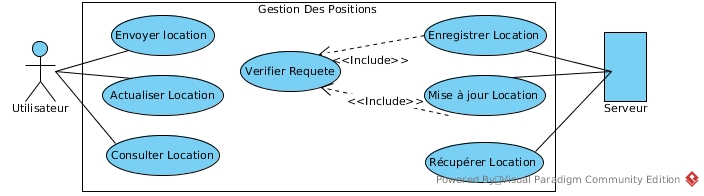
\includegraphics[width=1\textwidth]{sprint1-webservices-usecase}
  \caption{Diagram de case d'utilisation du services web en itération 1}
  \label{fig:sprint1-webservices-usecase}
\end{figure}

\begin{figure}[htbp]
  \centering
  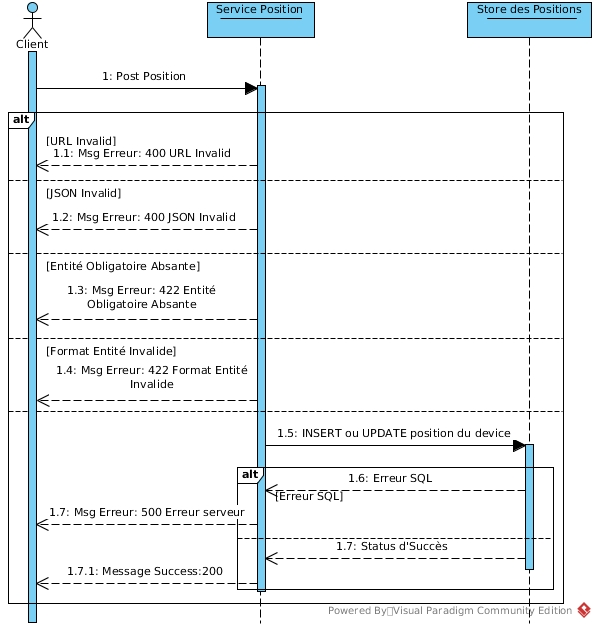
\includegraphics[width=1\textwidth]{sprint1-webservices-post-sequence}
  \caption{Diagram de sequence du service Post Postion en itération 1}
  \label{fig:sprint1-webservices-post-sequence}
\end{figure}

\begin{figure}[htbp]
  \centering
  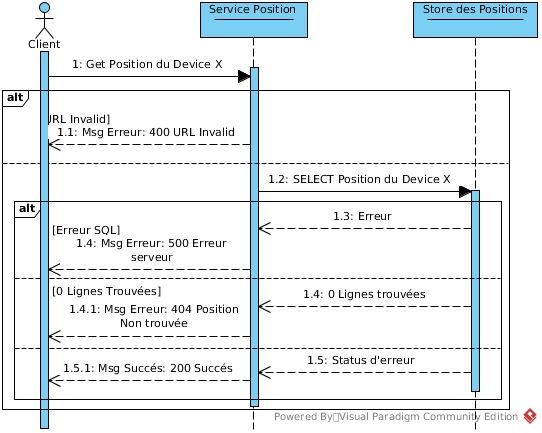
\includegraphics[width=1\textwidth]{sprint1-webservices-get-sequence}
  \caption{Diagram de sequence du service Get Postion en itération 1}
  \label{fig:sprint1-webservices-get-sequence}
\end{figure}

\subsection{Évaluation suivant les normes mise}
L’avis du Product-Owner sur notre première itération, nous a permis de commencer la
deuxième itération avec plus de confiance. Pour que nous puissions mieux nous
organiser, nous avons fait une petite étude

Ces caractéristique ont étés adressés pendant l'implémentation du service web.

\subsubsection{Performance}

On a minimisé la dépendance en bibliothèques externes et extensions PHP.
De plus, Le nombre des requêtes SQL ont étés minimisés à une seule requêtes pour
chaque méthode du notre service web.

\subsubsection{Multi-Utilisateurs}

Les positions à enregistrer doivent contenus un id qui doit etre utiliser aussi
pour retirer la dernière position.
On a utilisé diffèrent identificateur pour chaque périphériques basé sur le MAC
du phone.

\subsubsection{Portabilité}

On a utilisé la format standardisée JSON pour le transfert de données ce qui
assure que la portabilité des représentations des différents types des données
(nombres, booléens, strings, $\dotsc$) indépendant du localisation.

Pour le représentation des dates dans le content du requêtes HTTP, on a utilisé
la format RFC3339 \cite{RFC3339} avec UTC comme la défaut zone du temps, ex:
\verb|2005-08-15T15:52:01|.

Pour les en-têtes du requêtes HTTP, la format de représentation des dates est
RFC1123 \cite{RFC1123}, ex: \verb|Mon, 15 Aug 2005 15:52:01 +0000|.

La format du présentation des positions géologique (latitude et longitude)
choisi est la même représentation des nombres en JSON avec une précision jusqu'à
14 chiffres après le virgule. Les valeurs envoyés doivent respecte l'intervalle
des diffèrent entités géologiques ($latitude \in [-90, 90]$,
$longitude \in [-180, 180]$)

\subsubsection{Fiabilité}

Pour assuré la fiabilité d'un service web, on doit vérifier la validité de
contenu reçu même si envoyé depuis un source de confiance avant de les
utiliser. La vérification inclue le test de disponibilité des entités
obligatoires et le test de leurs formats.

\subsubsection{Implémenté la méthode POST}

Dans 1\ier{} phase, on a implémenté la méthode POST du ressource Position.
La documentation de l'api est dans l'annex~\ref{appendix:sprint1-position-post-doc}.

\subsubsection{Implementé la Méthod Get}

La documentation de l'api est dans l'annex~\ref{appendix:sprint1-position-get-doc}.

\TODO{RESTful API design describtion as http-api-design-en.pdf}

\subsection{Revue de cette itération}
\subsubsection{Produit de l'itération}

A la fin de l’itération 1, nous avons un première produit partiel permettant de 
suivre la position des multiple smartphone et les afficher dans la carte
maps de notre site web.

\paragraph{Page Web ``Dashboard''}

La figure \ref{fig:sprint1-dashboard-screenshot} affiche la position des individus et son état.
\begin{itemize}
 \item \textit{Marqueur en Vert}: Périphérique en ligne  
 \item \textit{Marqueur en Rouge}:Périphérique en hors ligne 
\end{itemize}

\begin{figure}[htbp]
  \centering
  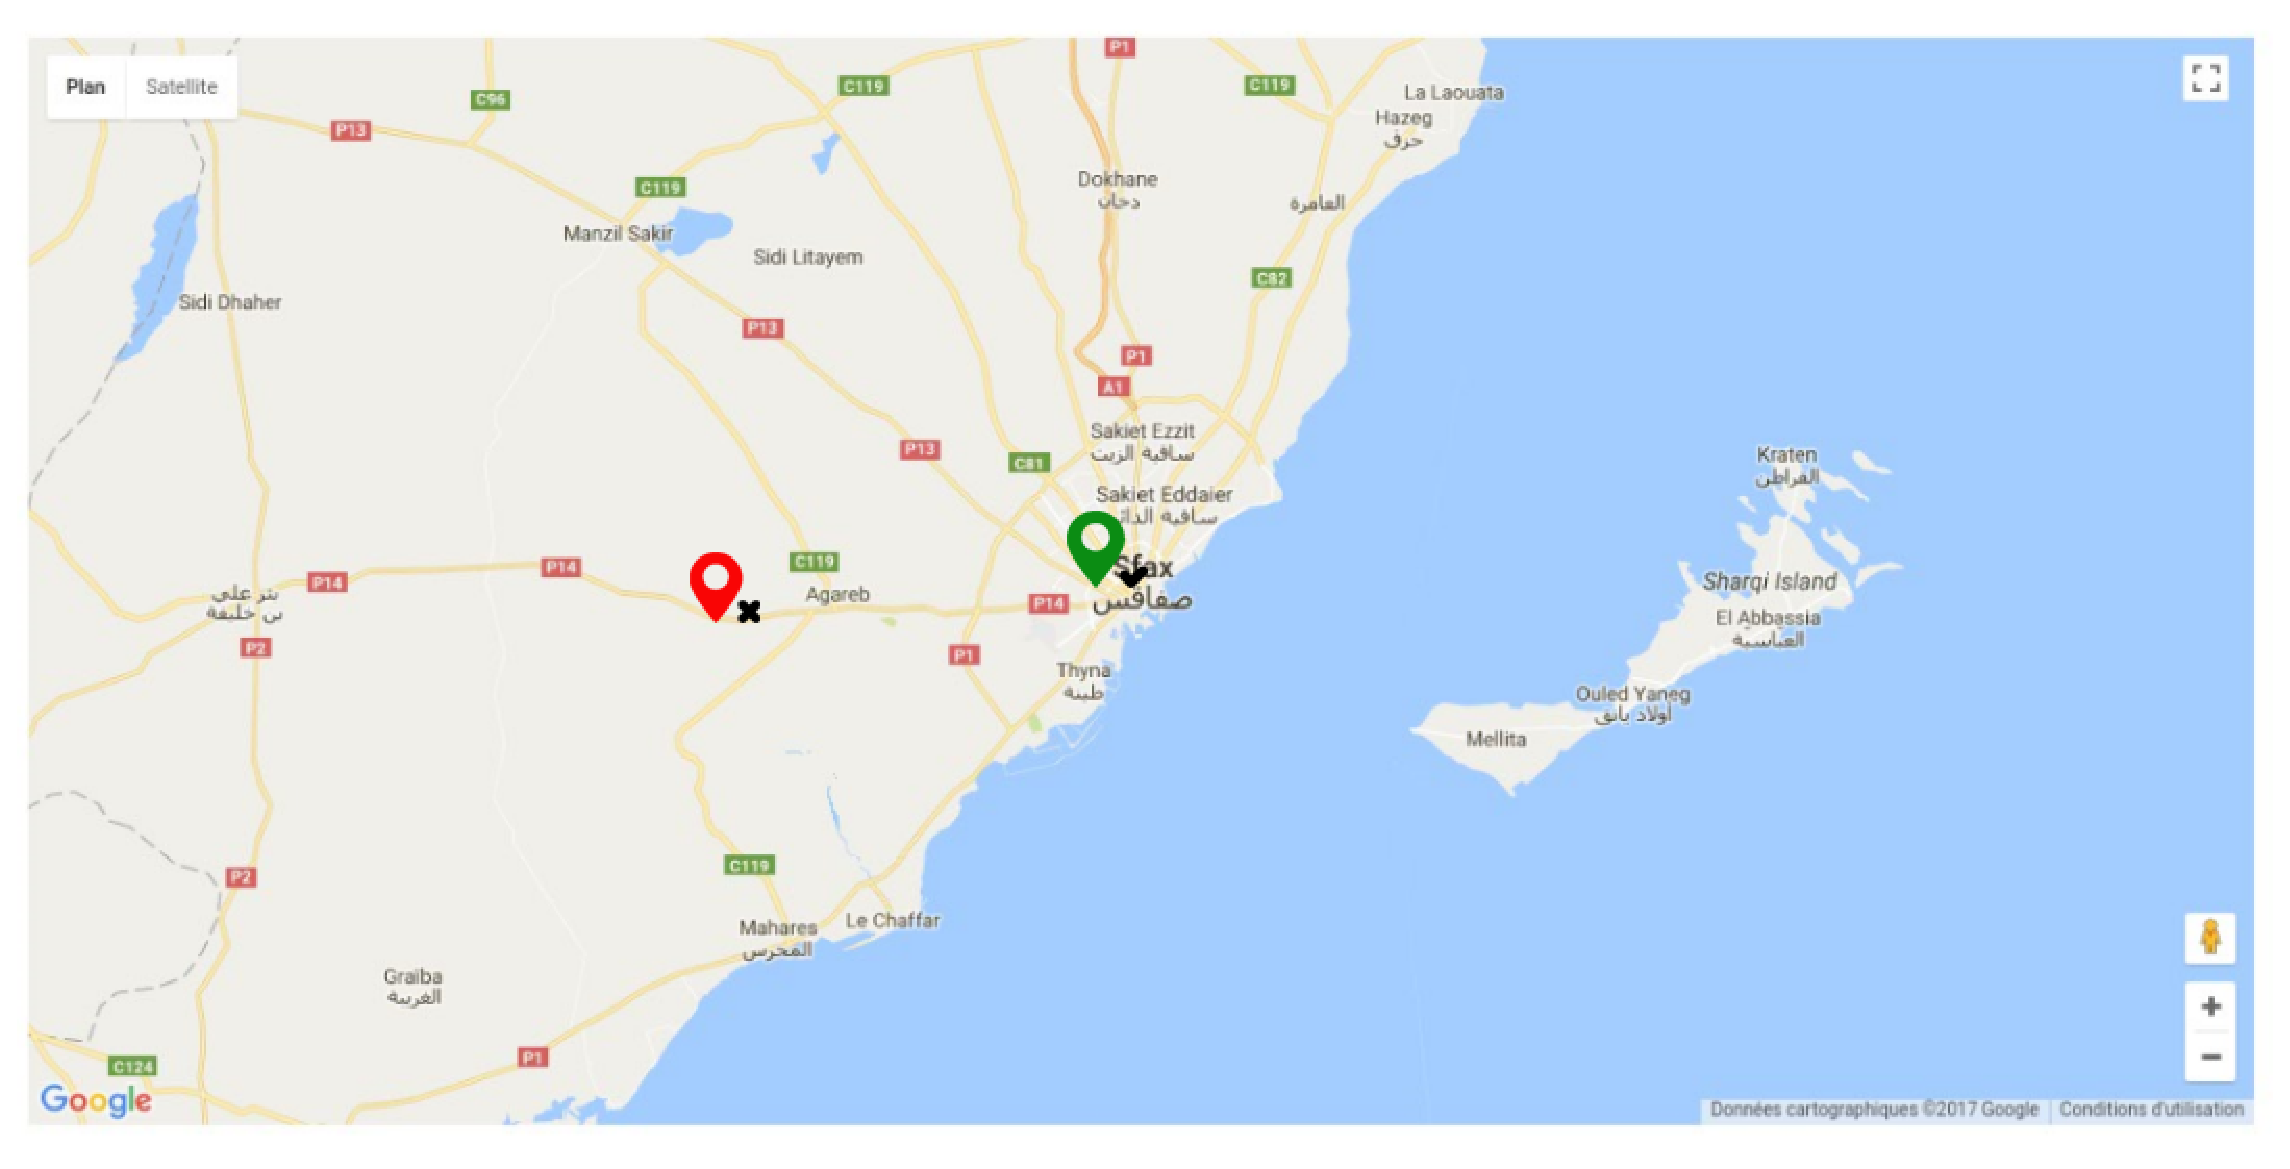
\includegraphics[width=0.6\textwidth]{sprint1-dashboard-screenshot}
  \caption{Capture écran de la page web de l'itération 1}
  \label{fig:sprint1-dashboard-screenshot}
\end{figure}

\paragraph{Application Android}

La figure \ref{fig:sprint1-android-screenshot} représente l'interface de l'application 
\begin{figure}[htbp]
  \centering
  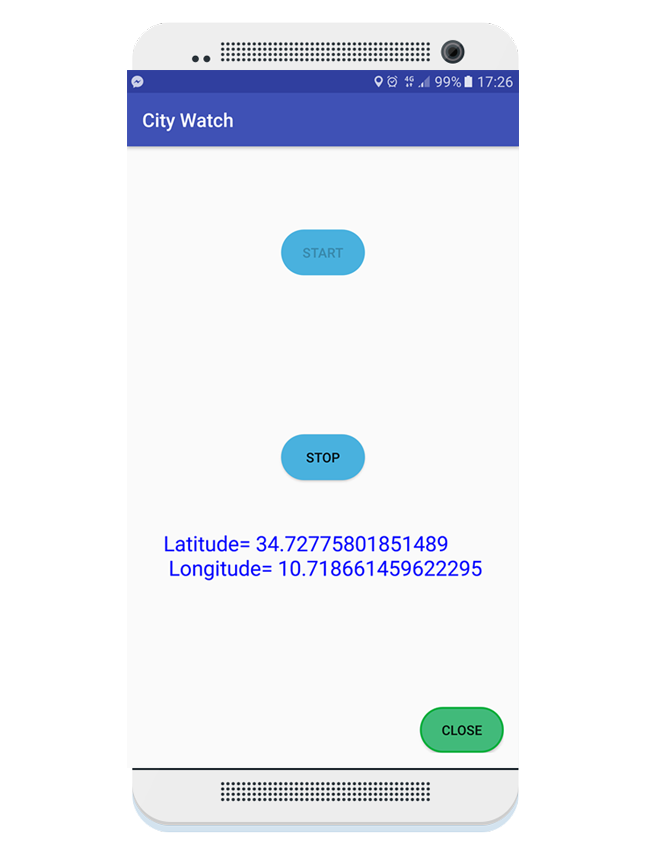
\includegraphics[width=0.4\textwidth]{sprint1-android-screenshot}
  \caption{Capture écran d'application Android de l'itération 1}
  \label{fig:sprint1-android-screenshot}
\end{figure}

\subsubsection{Avis du ProductOwner}

Le Product Owner était ravi des résultats de cette première itération. Il a validé donc notre
travail et nous a encouragé pour l’élaboration des suivantes itérations.

\subsection{Burndown de l'itération}

\usetikzlibrary{plotmarks}

\begin{figure}
\centering
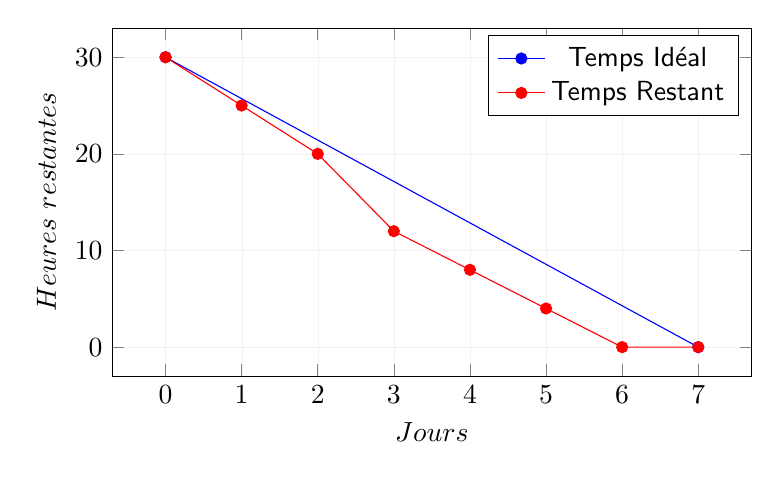
\begin{tikzpicture}[y=.2cm, x=.7cm,font=\sffamily]
\begin{axis}[
xlabel=$Jours$,
ylabel=$Heures\ restantes$,
grid=both,
grid style={line width=.1pt, draw=gray!10},
width=0.8\textwidth,
height=6cm,
%major grid style={line width=.2pt,draw=gray!50},
]
\addplot[color=blue,mark=*] coordinates {
        (0,30)
        (7, 0)
    };
    \addlegendentry{Temps Idéal}

    \addplot[mark=*,red] plot coordinates {
        (0, 30)
        (1, 25)
        (2, 20)
        (3, 12)
        (4, 8)
        (5, 4)
        (6, 0)
        (7, 0)
    };
    \addlegendentry{Temps Restant}
\end{axis}
\end{tikzpicture}
\caption{Graphique d'avancement - Itération 1}
\end{figure}

